\documentclass[12pt]{article}

\usepackage[utf8]{inputenc}
\usepackage{xcolor}
\usepackage[plainruled,noline]{algorithm2e}
\usepackage{graphicx}
\usepackage{subfig}

\definecolor{myred}{rgb}{1, 0, 0}
\definecolor{myblue}{rgb}{0.22, 0.42, 0.63}

% --------- Todos and remarks
\newcommand\todo[1]{\textcolor{blue}{TODO: #1}}

% --------- typography
\newcommand\func[1]{\textsl{#1}}
\newcommand\parentheses[1]{\big( #1 \big)}
\newcommand\brackets[1]{\big[ #1 \big]}


% --------- miscellaneous
\newcommand\AMi{AMi}

% --------- algorithm2e
\SetKwProg{Fn}{def}{\string:}{}
\SetKwFunction{FComputeAMiInterferences}{\textnormal{\func{ComputeAMiInterferences}}}
\SetKwFunction{FInstructions}{\textnormal{\func{Instructions}}}
\SetKwFunction{FIsPersistent}{\textnormal{\func{IsPersistent}}}
\SetKwFunction{FBasicBlocks}{\textnormal{\func{BasicBlocks}}}
\SetKwFunction{FBasicBlock}{\textnormal{\func{BasicBlock}}}
\SetKwFunction{FConnected}{\textnormal{\func{Connected}}}
\SetKwFunction{FIsUse}{\textnormal{\func{IsUse}}}
\SetKwFunction{FIsDef}{\textnormal{\func{IsDef}}}
\SetKwFunction{FUsers}{\textnormal{\func{Users}}}
\SetKwFunction{FEdge}{\textnormal{\func{Edge}}}
\SetKwFunction{FIndex}{\textnormal{\func{Index}}}
\SetKwFunction{FOperands}{\textnormal{\func{Operands}}}
\SetKwFunction{FDef}{\textnormal{\func{Def}}}
\SetKwFunction{FLiveAt}{\textnormal{\func{LiveAt}}}
\SetKwFunction{FDefines}{\textnormal{\func{Defines}}}
\SetKw{Assert}{assert}
\SetKwFor{For}{for}{}{}
\SetKwSwitch{Switch}{Case}{Other}{switch}{}{case}{otherwise}{}{}
\SetKwIF{If}{ElseIf}{Else}{if}{}{else if}{else}{}%
\SetKwIF{If}{ElseIf}{Else}{if}{}{else if}{else}{}%
\SetKwInput{KwData}{Input}
\SetKwComment{Comment}{\# }{}


\begin{document}

\begin{figure}[t!]
  \centering
  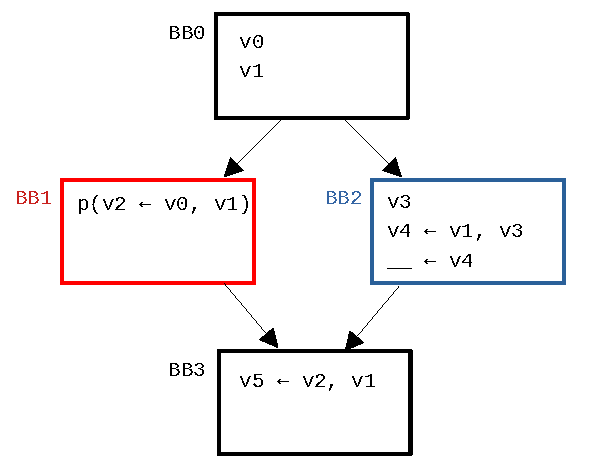
\includegraphics[width=0.5\textwidth]{cfg}
  \caption{\texttt{def-list} \brackets{\leftarrow\ \texttt{use-list}}}
\end{figure}

\begin{figure}[t!]
  \centering
  \subfloat[BB0 < \textcolor{myred}{BB1} < \textcolor{myblue}{BB2} < BB3]{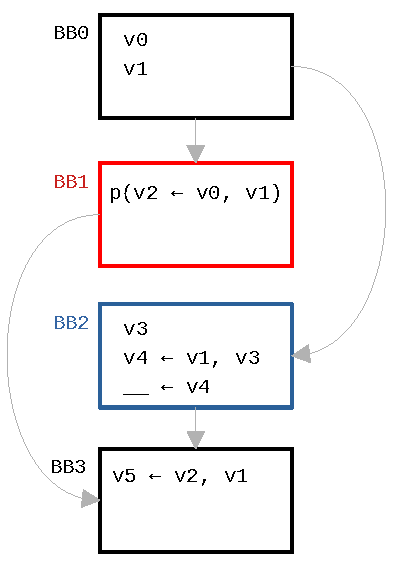
\includegraphics[width=0.35\textwidth]{lin1}} \hfill
  \subfloat[BB0 < \textcolor{myblue}{BB2} < \textcolor{myred}{BB1} < BB3]{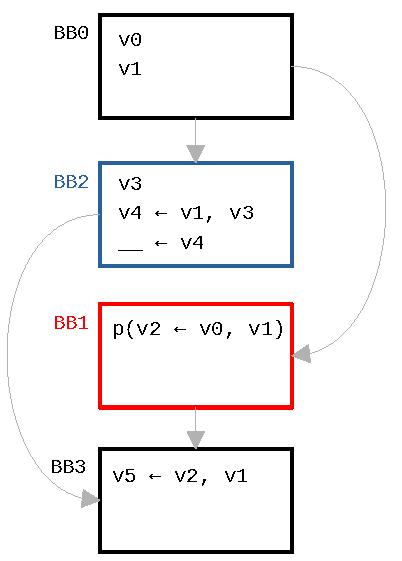
\includegraphics[width=0.35\textwidth]{lin2}}
  \caption{Linearization options}
  \label{fig:linearization-options}
\end{figure}

How to compute the \AMi-induced edges of the interference graph?

\section{Algorithm}

% Not in SSA (i.e., after phi-elimination)

% In a control-flow graph, a join point is a location where multiple control paths in the program converge.

% A secret-dependent region: (see also Libra paper for definition)
%     - A tuple of (set(basic block), set(dir-edge), entry, exit)
%     - Fully connected
%     - exit block postdominates all blocks
%     - terminator of entry is secret dependent

% - A linearization function defines a total order between instructions and
%    between basic blocks.
%    (LLVM linearization, *not* AMi linearization)
% => Index(i), Index(bb) are functions to retrieve the index of an instruction
%     and a basic block respectively within that order
%   Note that index(i) can be compared with Index(bb) (Abuse of notation?)
%
% - Users(R, i)
%       returns all users (instructions) of the register defined by
%         instruction i within region R
% - Operands(i)
%       returns all operands of the instruction
% - Operands(bb)
%       returns all operands of the instructions in a basic block
% - IsUse(op)
%       returns if the operand is a use
% - IsDef(op)
%       returns if the operand is a def
% - Def(op)
%       returns the defining instruction of the given operand
%          for SSA form this is a single instruction, for non-SSA form
%          this can be multiple instructions
% - LiveAt(v, bb)
%        return true if register v is live at bb
% - Instructions(R)
%       returns the instructions of the region R
% - Instructions(bb)
%       returns the instructions of the basic block bb
% - PersistentInstructions(R):
%       returns the persistent instructions of the region R
% - BasicBlock(i)
%       returns the basic block of the instruction i
% - Connected(bb1, bb2)
%        true if path from bb1 to bb2 or if path from bb2 to bb1
%              (bb2 is reachable from bb1 or bb1 is reachable from bb2)
% - Edge(u, v)
%        represents a directed edge from source u to target v

\setlength{\algomargin}{0em}

\begin{algorithm}
\Fn{\FComputeAMiInterferences{$R$}}{
  \DontPrintSemicolon
  %\SetCommentSty{\textcolor{blue}}
  \KwData{Secret-dependent region $R$}
  \KwResult{Set of \AMi-induced interference edges $E$}
  $E \gets \emptyset$\;
  \For{$p \in \FPersistentInstructions{R}$}{
    \For{$bb \in \FBasicBlocks{R} \mid \neg \FConnected(\FBasicBlock(p), bb)$}{

      \Comment{Case 1}
      \If{$\FIndex(bb) > \FIndex(\FBasicBlock(p))$}{

        \Comment{Case 1.1}
        \For{$user \in \FUsers(R, p)$}{
          \Assert{$\FIndex(user) < \FIndex(bb)\ \lor \FDefines(bb, p)$}\;
          \Comment{Else bug in \AMi{} tranformation?}
        }

        \Comment{Case 1.2}
        \For{$op \in \FOperands(bb) \mid \FIsUse(op)$}{
          \If{$\FIndex(\FDef(op)) < \FIndex(p)$}{
            $E \gets E \cup \{\FEdge(\FDef(op), p)\}$\;
            \Comment{LLVM: Add Segment(Range(p)) to LIS(Def(op))}
          } 
        }
      }

      \Comment{Case 2}
      \If{$\FIndex(bb) < \FIndex(\FBasicBlock(p))$}{

        \Comment{Case 2.1}
        \For{$op \in \FOperands(bb) \mid \FIsDef(op)$}{
          \For{$user \in \FUsers(\FDef(op)) \mid \FIndex(user) > \FIndex(p)$}{
            \Assert{$\FLiveAt(op, \FBasicBlock(p))$}\;
            \Comment{Else uninitialized var?}
          }
        }

        \Comment{Case 2.2}
        \For{$op \in \FOperands(p) \mid \FIsUse(op)$}{
          \If{$\FIndex(\FDef(op)) < \FIndex(bb)$} {
            \For{$i \in \FInstructions{bb}$} {
              $E \gets E \cup \{\FEdge(\FDef{op},i)\}$\;
              \Comment{LLVM: Add segment(bb) to LIS(p)}
              % TODO: Unless u already contains that slot index
            }
          }
        }
      }
    }
  }
  \Return{$E$}
}
\end{algorithm}

\todo{Add support for spilling and splitting.}

\end{document}
